
%(BEGIN_QUESTION)
% Copyright 2007, Tony R. Kuphaldt, released under the Creative Commons Attribution License (v 1.0)
% This means you may do almost anything with this work of mine, so long as you give me proper credit

Two wires lay parallel to each other inside an electrical conduit.  Through one of these wires runs a steadily increasing direct current:

$$\includegraphics[width=15.5cm]{i02403x01.eps}$$

Determine the following about the induced effect in the other wire:

\begin{itemize}
\item{} The direction of induced current in the second wire (please trace {\it conventional} flow!)
\vskip 10pt
\item{} The polarity of voltage drop across the resistor
\end{itemize}

Then, explain why the induced effects would be as you described, and not the other way (opposite direction, opposite polarity).

\underbar{file i02403}
%(END_QUESTION)





%(BEGIN_ANSWER)

$$\includegraphics[width=15.5cm]{i02403x02.eps}$$

The induced current runs opposite the incident current in accordance with Lenz's Law, in an attempt to oppose the change in magnetic flux near the wires.

%(END_ANSWER)





%(BEGIN_NOTES)


%INDEX% Electronics review: electromagnetic induction and Lenz's Law

%(END_NOTES)


